\documentclass{beamer}

%%% Работа с русским языком
\usepackage{cmap}					% поиск в PDF
\usepackage{mathtext} 				% русские буквы в формулах
\usepackage[T2A]{fontenc}			% кодировка
\usepackage[utf8]{inputenc}			% кодировка исходного текста
\usepackage[english,russian]{babel}	% локализация и переносы
\usepackage{indentfirst}
\frenchspacing

%%% Дополнительная работа с математикой
\usepackage{amsmath,amsfonts,amssymb,amsthm,mathtools} % AMS
\usepackage{icomma}

%%% Текст в колонки
\usepackage{multicol}

%%% Системы уравнений
\usepackage{cases}

%%% Таблицы
\usepackage{array}

%%% Картинки
\usepackage{graphicx}
\usepackage{float}

%%% Свои имена функций
\DeclareMathOperator{\Div}{div}
\DeclareMathOperator{\Const}{const}

%%% Список литературы
\usepackage{biblatex}
\ExecuteBibliographyOptions{url=false}
\addbibresource{../references.bib}

%%% Гиперссылки
\usepackage{hyperref}

%%% Перенос знаков в формулах (по Львовскому)
\newcommand*{\hm}[1]{#1\nobreak\discretionary{}
{\hbox{$\mathsurround=0pt #1$}}{}}


\usetheme{Madrid}
\title[Электрический пробой]{Моделирование электрического пробоя методом диффузной границы}
\author[]{Пономарев А.С. \\ под руководством Савенкова Е.Б., Зипуновой Е.В.}
\institute[]{группа Б05-029, 4 курс МФТИ}
\date{05.03.2024}
\logo{
\includegraphics[height=1cm]{../figures/ipm_label.jpg}}


\begin{document}

\begin{frame}
\titlepage
\end{frame}


\begin{frame}{Физическое явление}
\begin{block}{Электрический пробой}
	Явление резкого возрастания тока в диэлектрике при приложении электрического напряжения
	выше критического.
\end{block}
\begin{itemize}
	\item Рассматриваем твердый диэлектрик
	\item Деградация диэлектрических свойств материала
	\item Процесс развивается в ограниченной зоне -- канале
	\item Сложная физическая природа
\end{itemize}
\end{frame}


\begin{frame}{Математическая модель}
\begin{block}{Модель типа диффузной границы}
	Вещество находится в разных фазах. Состояние вещества приближается гладкой функцией
	$\phi(\omega, t)$ -- фазовым полем. Динамика процесса -- изменение фазового поля.
\end{block}
\begin{itemize}
	\item $\phi = 1$ -- неповрежденная среда
	\item $\phi = 0$ -- полностью разрушенная среда
	\item Зона $\phi \in (0, 1)$ -- диффузная граница
\end{itemize}
\end{frame}


\begin{frame}{Математическая модель}
Модель, предложенная в работе \cite{kiam_model}:
\begin{center}
	$\Omega \subset \mathbb{R}^3$ -- ограниченная область пространства \\
	$f(\phi) = 4 \phi^3 - 3 \phi^4$ -- интерполирующая функция
\end{center}
$$\epsilon(\omega, t) = \cfrac{\epsilon_0(\omega)}{f(\phi(\omega, t)) + \delta}$$
$$\Pi = \int \limits_\Omega \pi d \omega$$
$$\pi = -\cfrac{1}{2} \epsilon[\phi] (\nabla \Phi, \nabla \Phi) + \Gamma \cfrac{1 -
f(\phi)}{l^2} + \cfrac{\Gamma}{4} (\nabla \phi, \nabla \phi)$$
\end{frame}


\begin{frame}{Математическая модель}
\begin{block}{Уравнения модели}
	Уравнение электрического потенциала $\Phi$:
	$$\Div(\epsilon[\phi] \nabla \Phi) = 0 \label{equation_Phi}$$
	Уравнение фазового поля $\phi$:
	$$\cfrac{1}{m} \cfrac{\partial \phi}{\partial t} = \cfrac{1}{2} \epsilon'(\phi)
	(\nabla \Phi, \nabla \Phi) + \cfrac{\Gamma}{l^2} f'(\phi) +
	\cfrac{1}{2} \Gamma \triangle \phi$$
\end{block}
\end{frame}


\begin{frame}{Пример вычислительного эксперимента}
\begin{columns}
\column{0.32\textwidth}
\begin{figure}
	
\includegraphics[width=\textwidth]{../figures/model_example_1.png}
\end{figure}
\column{0.32\textwidth}
\begin{figure}
	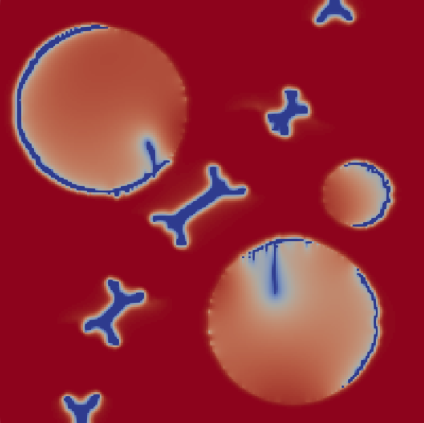
\includegraphics[width=\textwidth]{../figures/model_example_2.png}
\end{figure}
\column{0.32\textwidth}
\begin{figure}
	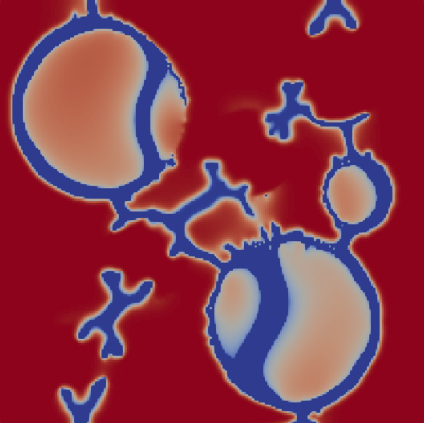
\includegraphics[width=\textwidth]{../figures/model_example_3.png}
\end{figure}
\end{columns}
\end{frame}


\begin{frame}{Одномерная задача}
$$\Omega = [0, w]_x \times [0, h]_y \times I_z$$
$$\Phi|_{y = 0} = \Phi^- \in \mathbb{R}, \quad \Phi|_{y = h} = \Phi^+ \in \mathbb{R}$$
Подходит функция электрического потенциала
$$\Phi(\omega, t) = \Phi^- \hm + \cfrac{y}{h}(\Phi^+ - \Phi^-)$$
Тогда уравнение на $\phi$ принимает вид
\begin{block}{}
	$$\cfrac{1}{m} \cfrac{\partial \phi}{\partial t} = \cfrac{1}{2} K_\Phi^2 \epsilon'(\phi) +
	\cfrac{\Gamma}{l^2} f'(\phi) + \cfrac{1}{2} \Gamma \cfrac{\partial^2 \phi}{\partial x^2}$$
\end{block}
Будем считать $\epsilon_0 = \Const$.
\end{frame}


\begin{frame}{Анализ положений равновесия}
Исследуем положения равновесия вида $\phi(x, t) \equiv C$. Положению равновесия соответствует
ноль $C$ функции
\vspace{-0.3cm}
$$\chi(\phi) = \cfrac{1}{2} K_\Phi^2 \epsilon'(\phi) + \cfrac{\Gamma}{l^2} f'(\phi)$$
\vspace{-0.8cm}
\begin{columns}
\column{0.3\textwidth}
\begin{figure}
	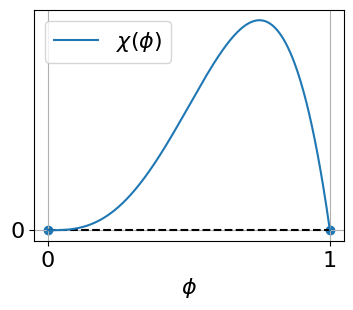
\includegraphics[width=\textwidth]{../figures/equilibriums_case_1.png}
\end{figure}
\vspace{-0.4cm}
$$0 \leq \cfrac{K_\Phi^2 l^2 \epsilon_0}{2 \Gamma} < \delta^2$$
\column{0.3\textwidth}
\begin{figure}
	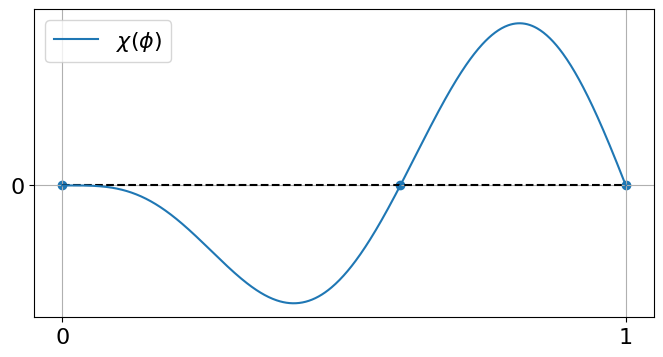
\includegraphics[width=\textwidth]{../figures/equilibriums_case_2.png}
\end{figure}
\vspace{-0.4cm}
$$\delta^2 < \cfrac{K_\Phi^2 l^2 \epsilon_0}{2 \Gamma} < (1 + \delta)^2$$
\column{0.3\textwidth}
\begin{figure}
	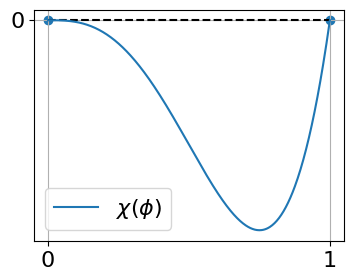
\includegraphics[width=\textwidth]{../figures/equilibriums_case_3.png}
\end{figure}
\vspace{-0.4cm}
$$(1 + \delta)^2 < \cfrac{K_\Phi^2 l^2 \epsilon_0}{2 \Gamma}$$
\end{columns}
\end{frame}


\begin{frame}{Анализ положений равновесия}
\vspace{-1cm}
\begin{columns}
\column{0.3\textwidth}
\begin{center}
	<<Слабое>> напряжение
\end{center}
\begin{figure}
	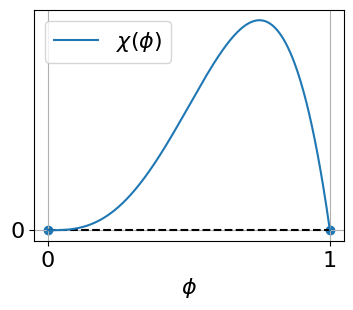
\includegraphics[width=\textwidth]{../figures/equilibriums_case_1.png}
\end{figure}
\column{0.3\textwidth}
\begin{center}
	<<Среднее>> напряжение
\end{center}
\begin{figure}
	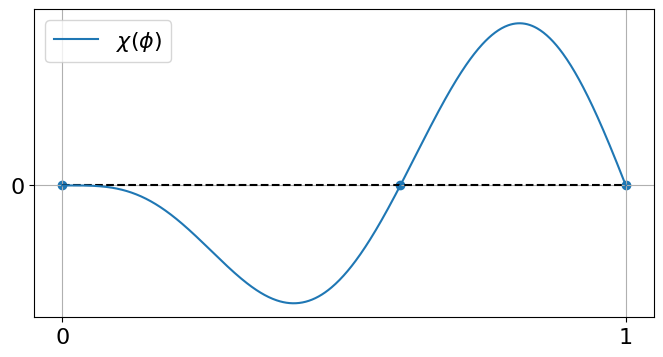
\includegraphics[width=\textwidth]{../figures/equilibriums_case_2.png}
\end{figure}
\column{0.3\textwidth}
\begin{center}
	<<Сильное>> напряжение
\end{center}
\begin{figure}
	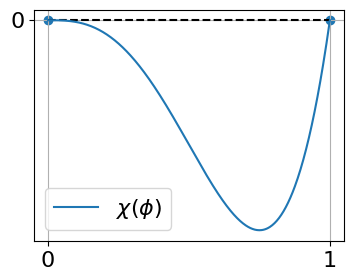
\includegraphics[width=\textwidth]{../figures/equilibriums_case_3.png}
\end{figure}
\end{columns}
\begin{columns}
\column{0.3\textwidth}
$\phi \equiv 0$ неустойчивое \\
$\phi \equiv 1$ устойчивое
\column{0.3\textwidth}
$\phi \equiv 0$ устойчивое \\
$\phi \equiv С_3$ неустойчивое \\
$\phi \equiv 1$ устойчивое
\column{0.3\textwidth}
$\phi \equiv 0$ устойчивое \\
$\phi \equiv 1$ неустойчивое
\end{columns}
\end{frame}


\begin{frame}{Разностная схема}
\begin{block}{Разностная задача}
	$$\cfrac{1}{m} \cfrac{\phi_a^{b + 1} - \phi_a^b}{\tau} = \cfrac{1}{2} K_\phi^2
	\epsilon'(\phi_a^b) + \cfrac{\Gamma}{l^2} f'(\phi_a^b) + \cfrac{\Gamma}{2}
	\cfrac{\phi_{a + 1}^b - 2 \phi_a^b + \phi_{a - 1}^b}{h^2}$$
	$$\phi_a^0 = \phi_0(ah); \quad \phi_0^b = \phi_l(b \tau); \quad \phi_{w/h}^b = \phi_r(b \tau)$$
	Сетка регулярная; $t$ -- шаг по времени, $h$ -- шаг по пространству.
\end{block}
Явная разностная схема первого порядка по времени, второго -- по пространству.
\end{frame}


\begin{frame}{Оценка устойчивости}
Рассмотрим возмущенное решение $\phi_a^b + \delta_a^b$. Линеаризуем уравнение на возмущение
$\delta_a^b$ в точке $\phi_a^b = P$:
$$\delta_a^{b + 1} = \delta_a^b + m \tau \left( \cfrac{1}{2} K_\Phi^2 \epsilon''(P) \delta_a^b +
\cfrac{\Gamma}{l^2} f''(P) \delta_a^b + \cfrac{\Gamma}{2} \cfrac{\delta_{a + 1}^b - 2 \delta_a^b +
\delta_{a - 1}^b}{h^2} \right)$$
Применим спектральный признак устойчивости:
$$1 > \lambda(\theta) = 1 + m \tau \left( \cfrac{1}{2} K_\Phi^2 \epsilon''(P) +
\cfrac{\Gamma}{l^2} f''(P) - \cfrac{2 \Gamma}{h^2} \sin^2 \cfrac{\theta}{2} \right)$$
Исследуем вблизи $0$.
\end{frame}


\begin{frame}{Оценка устойчивости}
\begin{block}{Условие устойчивости}
	$$\tau \leq \cfrac{1}{\cfrac{2.2 m K_\Phi^2 \epsilon_0}{\delta^{5/3}} +
	\cfrac{2m \Gamma}{h^2}}$$
\end{block}
\begin{block}{Упрощенное условие устойчивости}
	$$\tau \leq \min \left(\cfrac{\delta^{5/3}}{4.4 m K_\Phi^2 \epsilon_0}, \;
	\cfrac{h^2}{4m \Gamma} \right)$$
\end{block}
\end{frame}


\begin{frame}{Вычисления: типичное решение}
\begin{figure}
	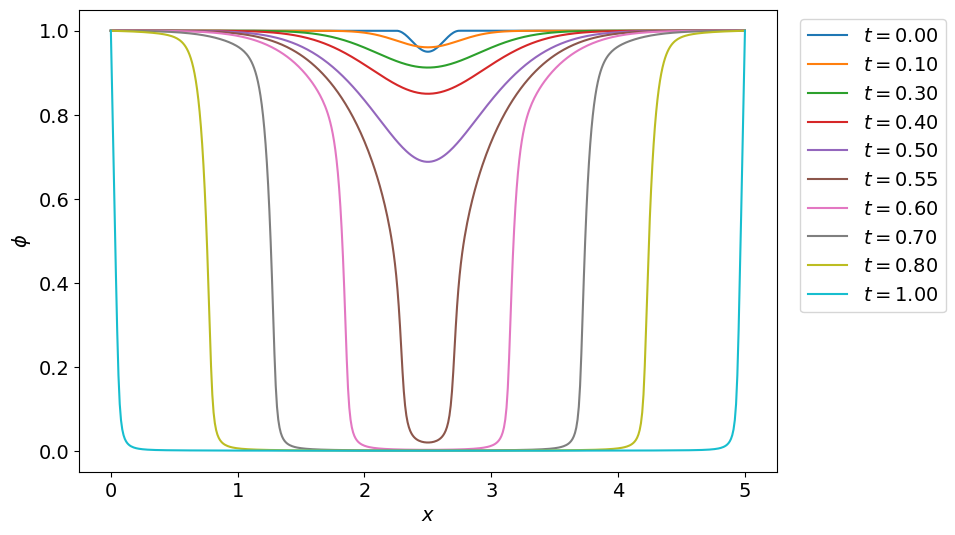
\includegraphics[width=\textwidth]{../figures/typical_solution.png}
\end{figure}
\vspace{-0.8cm}
\begin{center}
	Узлов по измерениям: $n_x = 10^3, \; n_t = 10^5$
\end{center}
\end{frame}


\begin{frame}{Вычисления: проверка устойчивости}
\vspace{-0.5cm}
\begin{figure}
	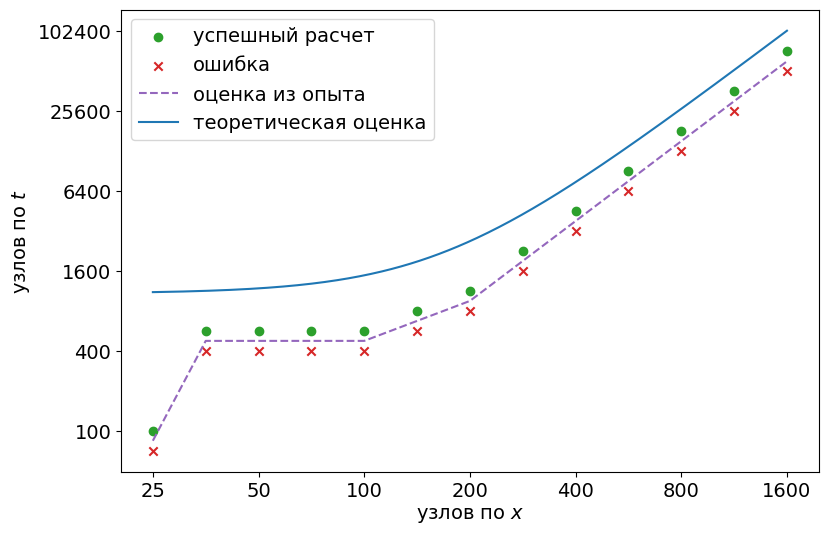
\includegraphics[width=0.8\textwidth]{../figures/stability_bounds.png}
\end{figure}
\vspace{-0.3cm}
$$\tau \leq \left( \cfrac{2.2 m K_\Phi^2 \epsilon_0}{\delta^{5/3}} +
\cfrac{2m \Gamma}{h^2} \right)^{-1}$$
\end{frame}


\begin{frame}{Вычисления: проверка сходимости}
Проводится ряд вычислений, затем результаты сравниваются по норме с лучшим в ряду.
\begin{columns}
\column{0.45\textwidth}
\begin{figure}
	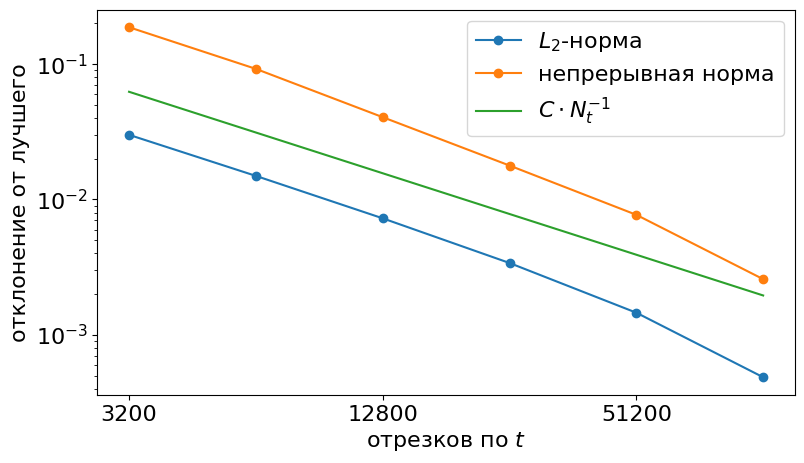
\includegraphics[width=\textwidth]{../figures/convergence_fixed_nx.png}
\end{figure}
\column{0.45\textwidth}
\begin{figure}
	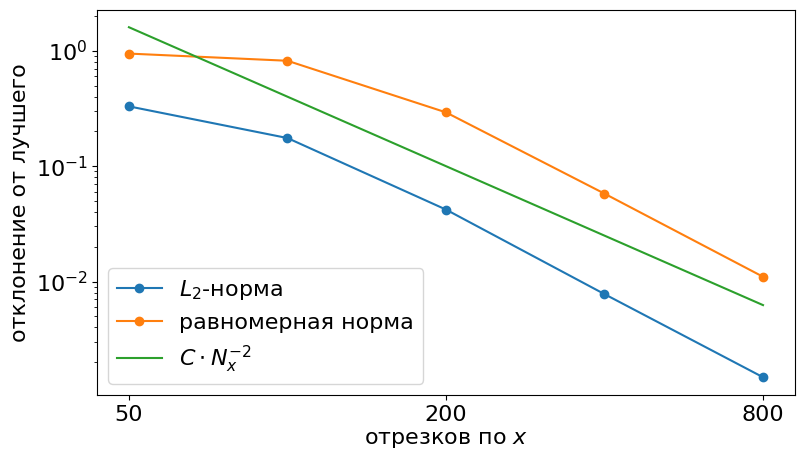
\includegraphics[width=\textwidth]{../figures/convergence_fixed_nt.png}
\end{figure}
\end{columns}
\end{frame}


\begin{frame}{Вычисления: проверка сходимости}
\vspace{-0.2cm}
\begin{figure}
	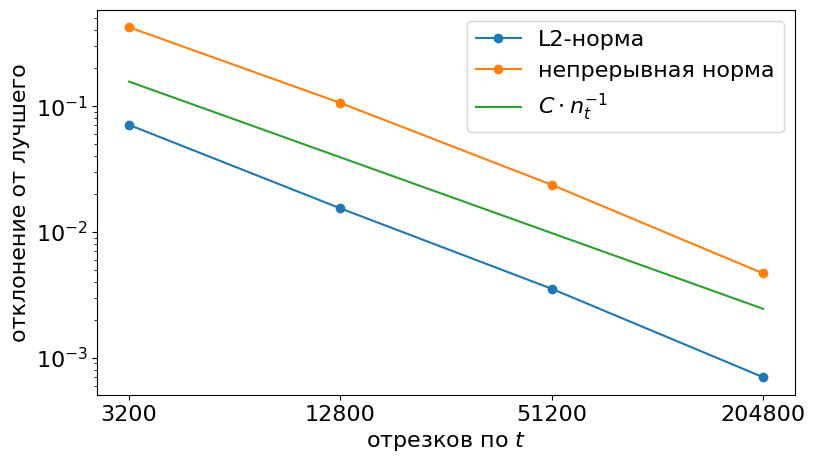
\includegraphics[width=0.75\textwidth]{../figures/convergence_connected.png}
\end{figure}
\vspace{-0.7cm}
\begin{center}
	Здесь, согласно оценке устойчивости, $\tau = \cfrac{h^2}{4m \Gamma}$.
\end{center}
\end{frame}


\begin{frame}{Вычисления: положения равновесия}
\begin{center}
	$0 \leq \cfrac{K_\Phi^2 l^2 \epsilon_0}{2 \Gamma} < \delta^2$ -- <<слабое>> напряжение
\end{center}
\begin{columns}
\column{0.45\textwidth}
\begin{figure}
	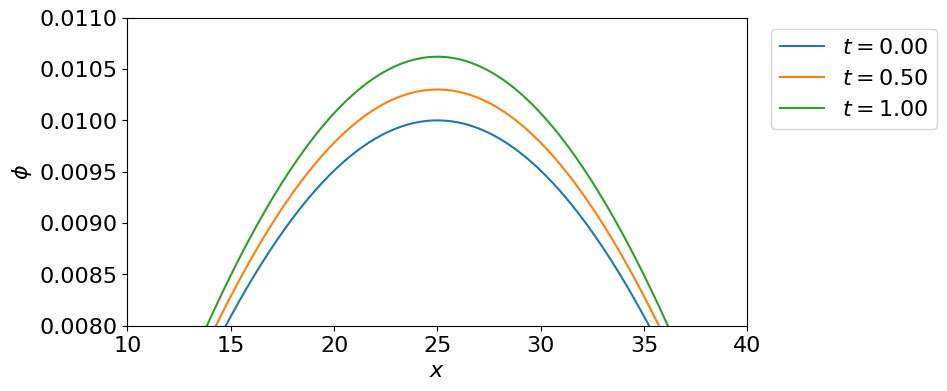
\includegraphics[width=\textwidth]{../figures/equilibrium_1_0.png}
\end{figure}
\begin{center}
	$\phi \equiv 0$ \\
	неустойчивое
\end{center}
\column{0.45\textwidth}
\begin{figure}
	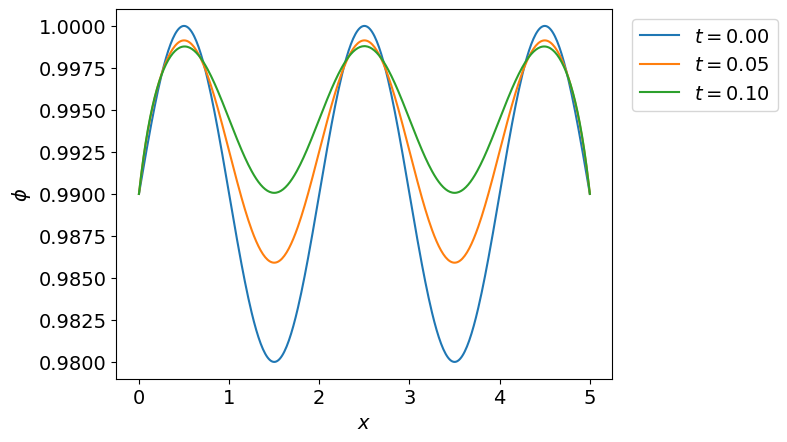
\includegraphics[width=\textwidth]{../figures/equilibrium_1_1.png}
\end{figure}
\begin{center}
	$\phi \equiv 1$ \\
	устойчивое
\end{center}
\end{columns}
\end{frame}


\begin{frame}{Вычисления: положения равновесия}
\begin{center}
	$\delta^2 < \cfrac{K_\Phi^2 l^2 \epsilon_0}{2 \Gamma} < (1 + \delta)^2$ --
	<<среднее>> напряжение
\end{center}
\begin{columns}
\column{0.33\textwidth}
\begin{figure}
	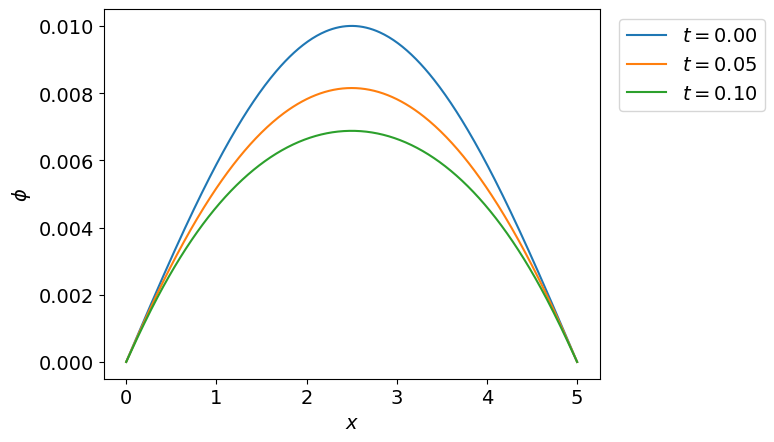
\includegraphics[width=\textwidth]{../figures/equilibrium_2_0.png}
\end{figure}
\begin{center}
	$\phi \equiv 0$ \\
	устойчивое
\end{center}
\column{0.33\textwidth}
\begin{figure}
	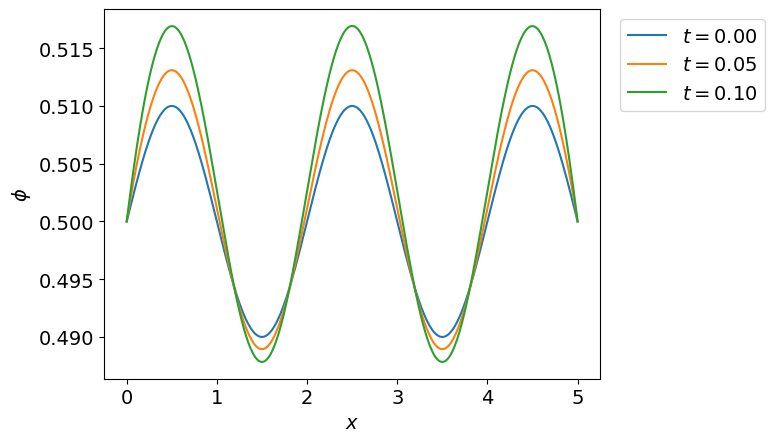
\includegraphics[width=\textwidth]{../figures/equilibrium_2_05.png}
\end{figure}
\begin{center}
	$\phi \equiv C_3$ \\
	неустойчивое
\end{center}
\column{0.33\textwidth}
\begin{figure}
	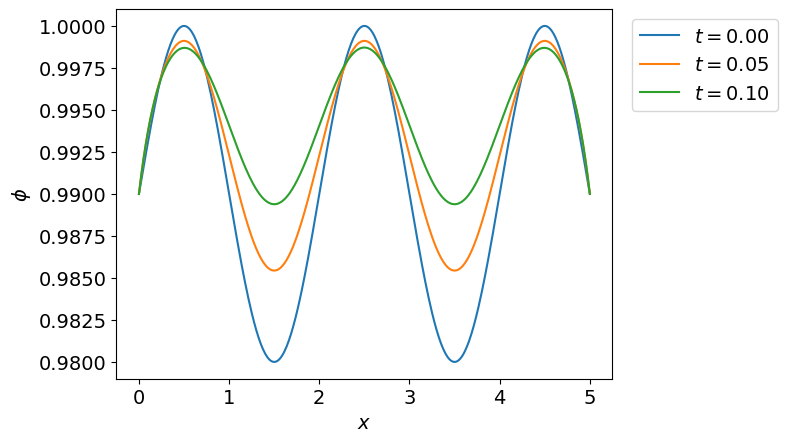
\includegraphics[width=\textwidth]{../figures/equilibrium_2_1.png}
\end{figure}
\begin{center}
	$\phi \equiv 1$ \\
	устойчивое
\end{center}
\end{columns}
\end{frame}


\begin{frame}{Вычисления: положения равновесия}
\begin{center}
	$(1 + \delta)^2 < \cfrac{K_\Phi^2 l^2 \epsilon_0}{2 \Gamma}$ -- <<сильное>> напряжение
\end{center}
\begin{columns}
\column{0.45\textwidth}
\begin{figure}
	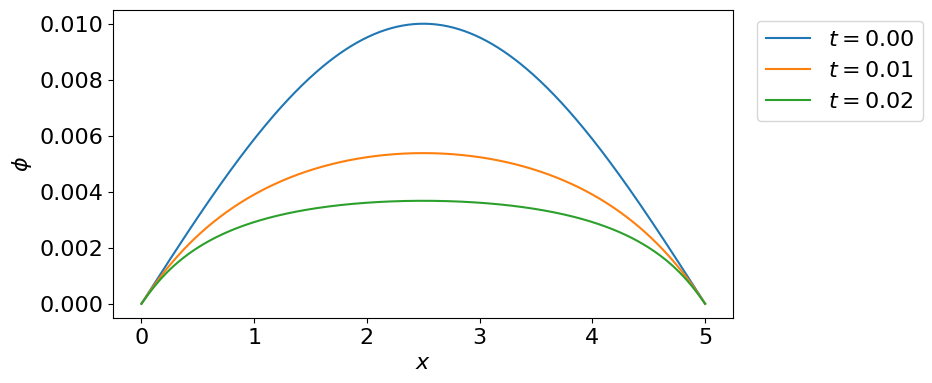
\includegraphics[width=\textwidth]{../figures/equilibrium_3_0.png}
\end{figure}
\begin{center}
	$\phi \equiv 0$ \\
	устойчивое
\end{center}
\column{0.45\textwidth}
\begin{figure}
	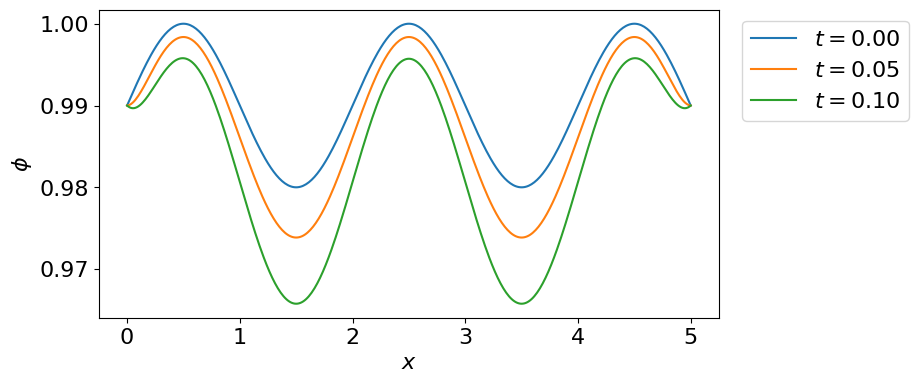
\includegraphics[width=\textwidth]{../figures/equilibrium_3_1.png}
\end{figure}
\begin{center}
	$\phi \equiv 1$ \\
	неустойчивое
\end{center}
\end{columns}
\end{frame}


\begin{frame}{Свободная энергия}
$$\Pi(t) = \int\limits_\Omega \pi(x, t) dx$$
$$\pi(x, t) = \pi_1(x, t) + \pi_2(x, t) + \pi_3(x, t)$$
$\pi_1(x, t) = -\cfrac{K_\Phi^2}{2} \, \epsilon(\phi(x, t))$ -- плотность энергии электрического
поля; \\
$\pi_2(x, t) = \Gamma \cfrac{1 - f(\phi(x, t))}{l^2}$ -- плотность энергии роста пробоя
в глубину; \\
$\pi_3(x, t) = \cfrac{\Gamma}{4} \left( \cfrac{\partial \phi}{\partial x}(x, t) \right)^2$ --
плотность энергии образования граничной зоны пробоя
\end{frame}


\begin{frame}{Вычисления: свободная энергия}
\begin{columns}
\column{0.5\textwidth}
\begin{figure}
	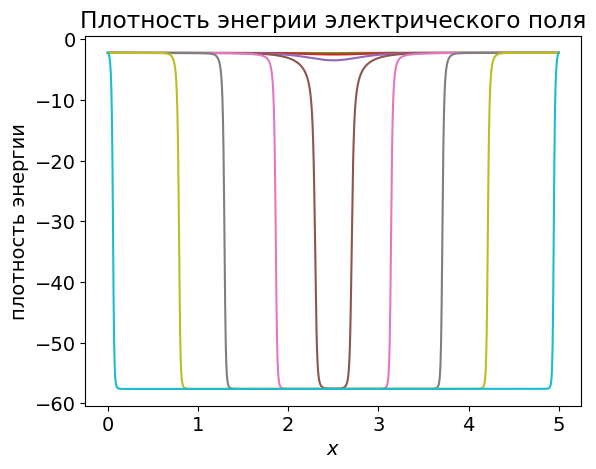
\includegraphics[width=\textwidth]{../figures/density_electrical.png}
\end{figure}
\begin{center}
	плотность энергии \\
	электрического поля
\end{center}
\column{0.5\textwidth}
\begin{figure}
	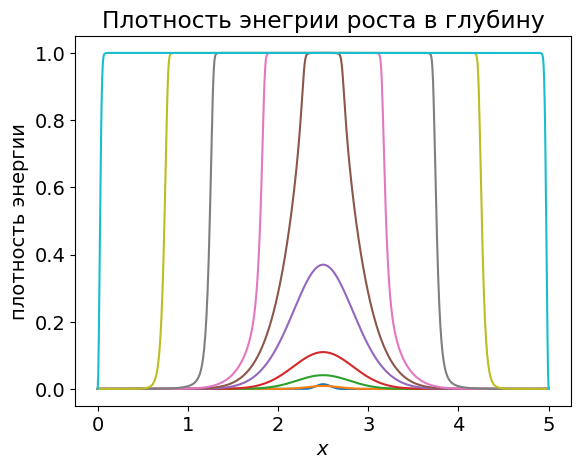
\includegraphics[width=\textwidth]{../figures/density_depth.png}
\end{figure}
\begin{center}
	плотность энергии \\
	роста в глубину
\end{center}
\end{columns}
\end{frame}


\begin{frame}{Вычисления: свободная энергия}
\begin{columns}
\column{0.5\textwidth}
\begin{figure}
	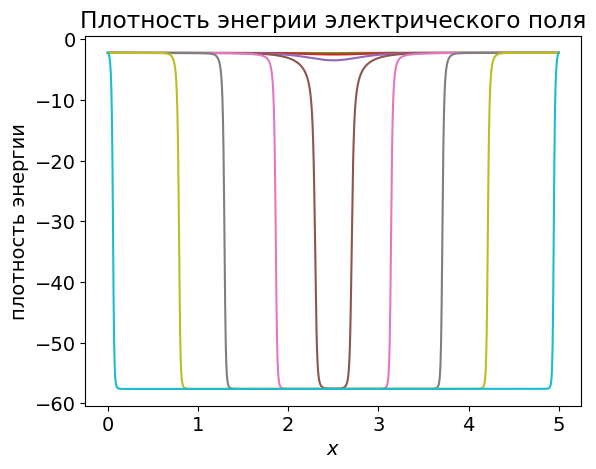
\includegraphics[width=\textwidth]{../figures/density_electrical.png}
\end{figure}
\column{0.5\textwidth}
\begin{figure}
	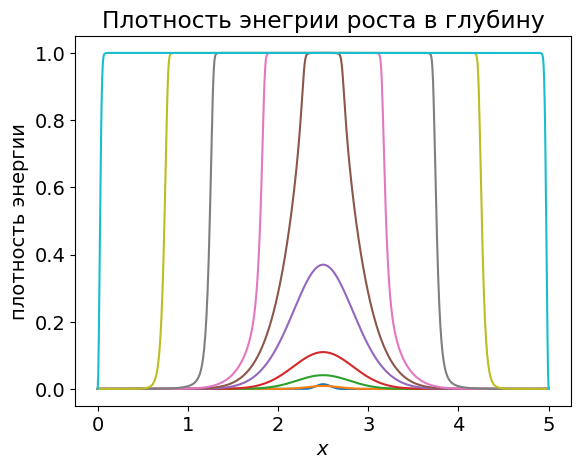
\includegraphics[width=\textwidth]{../figures/density_depth.png}
\end{figure}
\end{columns}
\end{frame}


\begin{frame}{Вычисления: свободная энергия}
\vspace{-0.3cm}
\begin{figure}
	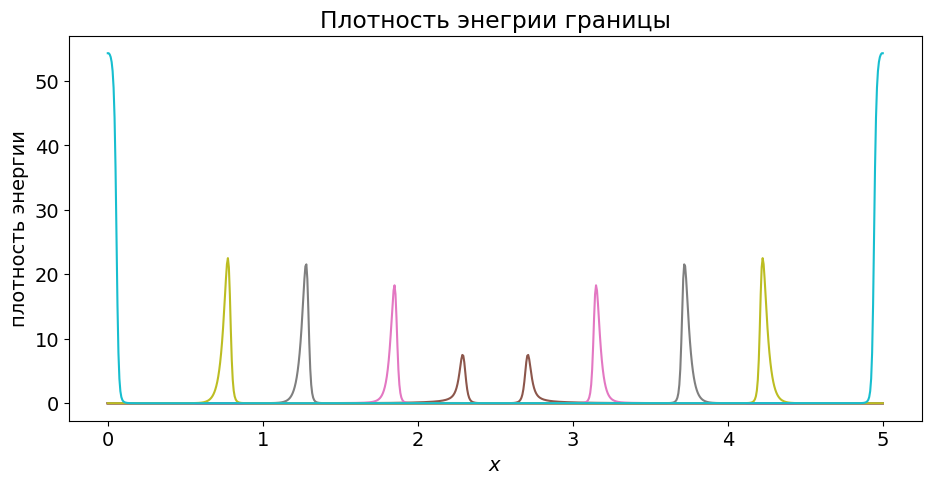
\includegraphics[width=0.65\textwidth]{../figures/density_surface.png}
\end{figure}
\vspace{-0.4cm}
\begin{figure}
	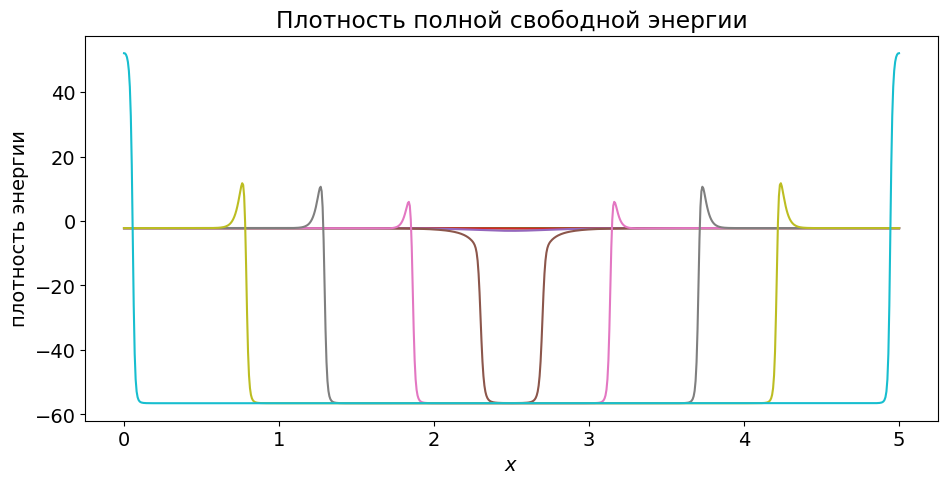
\includegraphics[width=0.65\textwidth]{../figures/density_total.png}
\end{figure}
\end{frame}


\begin{frame}{Вычисления: свободная энергия}
\begin{figure}
	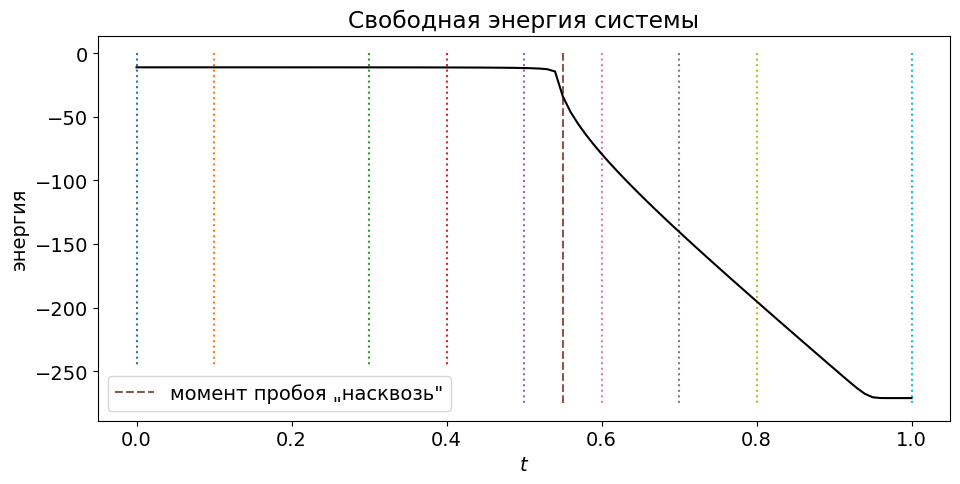
\includegraphics[width=\textwidth]{../figures/energy_total.png}
\end{figure}
\end{frame}


\begin{frame}{Литература}
\printbibliography
\end{frame}


\end{document}